\documentclass{standalone}
%% package needed
\usepackage{pgfplots}
\usepackage{anyfontsize}
\pgfplotsset{compat=newest}
\usetikzlibrary{positioning,arrows}

\newlength{\tracewidth} \setlength{\tracewidth}{12cm}
\newlength{\lwidth}     \setlength{\lwidth}    {3pt}


%% begin the document which is only a TikZ picture
%% -----------------------------------------------
\begin{document}
%% -----------------------------------------------
%% begin the TikZ picture

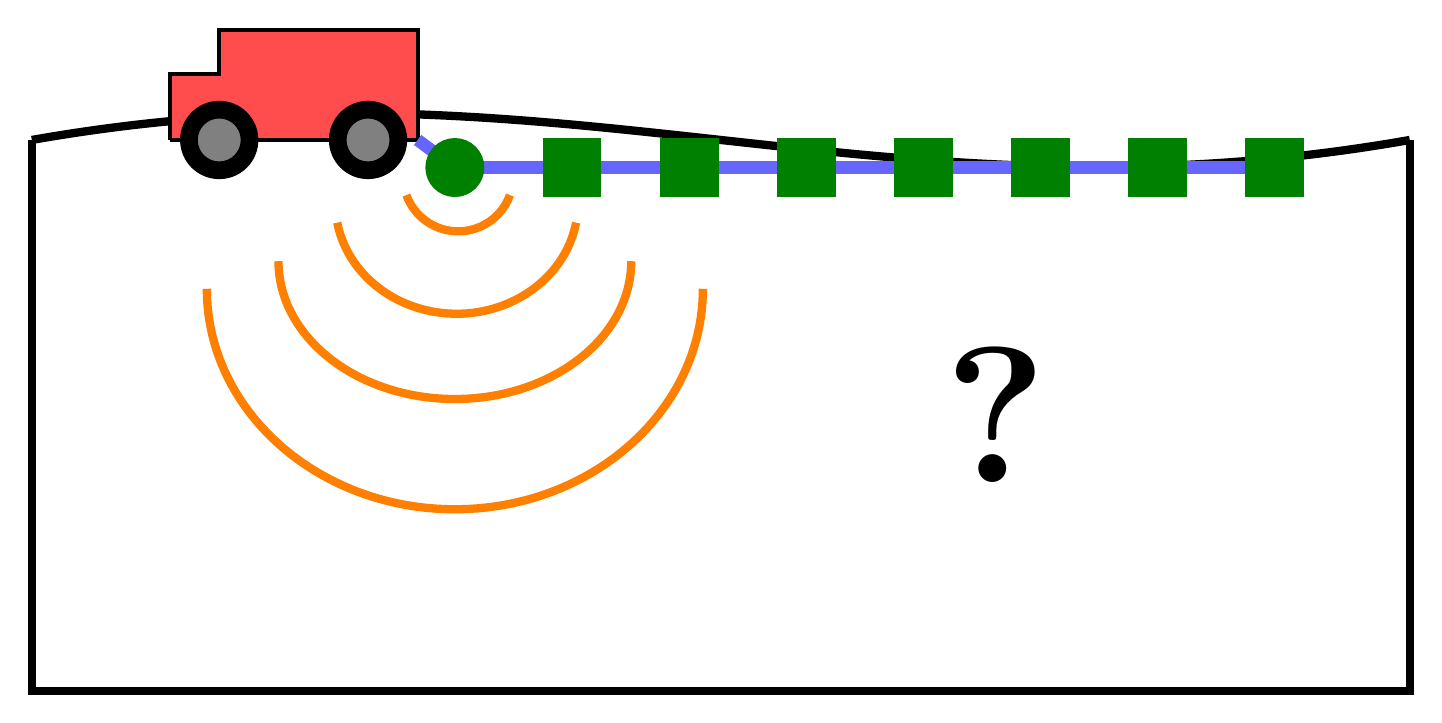
\begin{tikzpicture}[scale=7.]
  %% domain as a 2D rectangle
  %% ------------------------------------
  \pgfmathsetmacro{\xlength}{2.5}
  \pgfmathsetmacro{\ylength}{1}
  \coordinate (f4) at (0,\ylength); \coordinate (f3) at (\xlength,\ylength);
  \coordinate (f1) at (0,0)       ; \coordinate (f2) at (\xlength,0);
  \draw      [line width=\lwidth] (f4)--(f1)--(f2)--(f3);
  \draw (f4) [line width=\lwidth,out=10,in=-170] to[] (f3);

  %% Truck
  %% ------------------------------------
  \pgfmathsetmacro{\bposx}{0.1*\xlength} \pgfmathsetmacro{\bsx}{.45}
  \pgfmathsetmacro{\bposy}{1.0*\ylength} \pgfmathsetmacro{\bsy}{.20}
  \coordinate (b1)at (\bposx         ,\bposy);
  \coordinate (b2)at (\bposx+\bsx    ,\bposy);
  \coordinate (b3)at (\bposx+\bsx    ,\bposy+\bsy);
  \coordinate (b4)at (\bposx+0.2*\bsx,\bposy+\bsy);
  \coordinate (b5)at (\bposx+0.2*\bsx,\bposy+0.6*\bsy);
  \coordinate (b6)at (\bposx         ,\bposy+0.6*\bsy);
  \draw [line width=.5\lwidth,fill=red!70!white] (b1)--(b2)--(b3)--(b4)--(b5)--(b6)--(b1);
  %% Wheel
  \coordinate (w1)at (\bposx+0.2*\bsx,\bposy);
  \coordinate (w2)at (\bposx+0.8*\bsx,\bposy);
  \draw[fill=black](w1) circle (0.07) ;
  \draw[fill=black](w2) circle (0.07) ;
  \draw[fill=gray] (w1) circle (0.04) ;
  \draw[fill=gray] (w2) circle (0.04) ;

  %% towed streamer
  %% ------------------------------------
  \pgfmathsetmacro{\sx}{\bposx+1.15*\bsx}
  \pgfmathsetmacro{\sz}{0.95*\bposy}
  \coordinate (s1)at (b2);
  \coordinate (s2)at (\sx,\sz);
  \draw [line width=1.5\lwidth,blue!60!white](s1)--(s2);

  %% Sources and receivers
  %% -------------------------------------
  \pgfmathsetmacro{\rstep}{0.085*\xlength}
  \coordinate (r1)at (\sx + 1*\rstep,\sz);
  \coordinate (r2)at (\sx + 2*\rstep,\sz);
  \coordinate (r3)at (\sx + 3*\rstep,\sz);
  \coordinate (r4)at (\sx + 4*\rstep,\sz);
  \coordinate (r5)at (\sx + 5*\rstep,\sz);
  \coordinate (r6)at (\sx + 6*\rstep,\sz);
  \coordinate (r7)at (\sx + 7*\rstep,\sz);
  \draw[mark=*,mark size=.4\lwidth,mark options={color=green!50!black},
        blue!60!white,line width=1.5\lwidth]
        %% Source
        plot coordinates{(s2)}
        %% Receivers
     -- plot[mark=square*,mark size=.4\lwidth]
             coordinates {(r1)}
     -- plot[mark=square*,mark size=.4\lwidth,mark options={color=green!50!black}]
             coordinates {(r2)}
     -- plot[mark=square*,mark size=.4\lwidth] coordinates {(r3)}
     -- plot[mark=square*,mark size=.4\lwidth] coordinates {(r4)}
     -- plot[mark=square*,mark size=.4\lwidth] coordinates {(r5)}
     -- plot[mark=square*,mark size=.4\lwidth] coordinates {(r6)}
     -- plot[mark=square*,mark size=.4\lwidth] coordinates {(r7)};
 %% wave
 %% -------------------------------------
 \draw[orange,line width=\lwidth] (\sx+0.10,\sz-0.05) arc (-20:-160:0.10) ;
 \draw[orange,line width=\lwidth] (\sx+0.22,\sz-0.10) arc (-10:-170:0.22 and 0.20) ;
 \draw[orange,line width=\lwidth] (\sx+0.32,\sz-0.17) arc (  0:-180:0.32 and 0.25) ;
 \draw[orange,line width=\lwidth] (\sx+0.45,\sz-0.22) arc (  0:-180:0.45 and 0.40) ;

 %% legend
 %% ------------------------------------------------------------
 \node[anchor=center] (Qmark)  at (.7*\xlength,.5*\ylength){{\fontsize{70}{80}\selectfont \textbf{?}}};

\end{tikzpicture}

%% \hspace{5cm}
%% \begin{tikzpicture}
%%    \begin{axis}[
%%    width=     \tracewidth,
%%    height=0.75\tracewidth,
%%    axis on top, separate axis lines,
%%    xmin=0.0, xmax=183,  %xlabel={\huge receiver position (km)},
%%    ymin=0.0, ymax=2600, ylabel={{\fontsize{32}{42}\selectfont time} }, y dir=reverse,
%%    yticklabels={,,},xticklabels={,,}]
%%    \addplot [forget plot] graphics [xmin=0,xmax=183,ymin=0,ymax=2600] {./trace.png};
%%    \end{axis}
%% \end{tikzpicture}
%% ----------------------
\end{document}
